\documentclass{kththesis}

\justifying

\usepackage{graphicx}

\usepackage{bm}

% remove this if you are using XeLaTeX or LuaLaTeX
\usepackage[utf8]{inputenc}

% Use natbib abbreviated bibliography style
\usepackage[square,numbers]{natbib}
\bibliographystyle{unsrtnat}

\usepackage{lipsum} % This is just to get some nonsense text in this template, can be safely removed

\title{Sequential User Retention Modelling}
\alttitle{Detta är den svenska översättningen av titeln}
\author{Helder Martins}
\email{helder@kth.se}
\supervisor{Hedvig Kjellström (KTH) and Sahar Asadi (Spotify)}
\examiner{Patric Jensfelt}
\programme{Master in Machine Learning}
\school{School of Computer Science and Communication}
\date{\today}


\begin{document}

% Title page
\flyleaf

\begin{abstract}
  English abstract goes here.
\end{abstract}

\clearpage

\begin{otherlanguage}{swedish}
  \begin{abstract}
    Träutensilierna i ett tryckeri äro ingalunda en faktor där
    trevnadens ordningens och ekonomiens upprätthållande, och dock är
    det icke sällan som sorgliga erfarenheter göras ordningens och
    ekon och miens därmed upprätthållande. Träutensilierna i ett
    tryckeri äro ingalunda en oviktig faktor, för trevnadens
    ordningens och och dock är det icke sällan.
  \end{abstract}
\end{otherlanguage}

\cleardoublepage

\tableofcontents


% This is where the actual contents of the thesis starts
\mainmatter


\chapter{Introduction}

	This chapter will be dedicated to introduce the topic of this thesis project, the motivations on why it is relevant to both academia and to the industry, the current context where this project is being developed on, the hypothesis that shall be explored, the methodology used to verify it, and the contributions of this work.
	
	The rise of streaming services has in recent years revolutionized the way customers get access to digital content. The traditional model of media ownership, even though it still represents a significant share of revenue, is continuously losing ground to a new right-of-access model where users get access to content ether by paying a monthly subscription or by being exposed to advertisement. The customer base of said services is steadily growing, and with it the amount data collected tracking how they interact with the provided digital media. This information is of high-value to any provider who expects improve the user experience, increase its total number of clients and also avoid losing the current ones to the competition.
	
	One application of a data set like this that has received attention from the industry is to predict the clients that are more likely to leave the service in the near future and anticipate it by performing a set of actions with the goal of avoiding it from happening. It is predicted that there are a set of features which are highly correlated with their desire of abandoning the application, and thus a model could be trained to leverage this information and classify users based on the probability of that even occurring. Such models are called \emph{churn predictors}, and will be a central subject on this thesis project. Another interest will be to evaluate which set of features among the available ones actually correlates with churn and extract from it actionable insights that can be suggested to the provider as a form of improvement to their application, a task made harder by the extremely large number of attributes that is commonly captured.
	 
	The user behaviour data and the required computational resources were provided by \emph{Spotify}, a well known music streaming service that joined this project in a tutoring partnership with the student and the university. Creating a suitable data set for training our proposed models is also part of the project, and it was performed by first exploring the data at our disposal and identifying the features that highly correlates with churn. While the available data is mostly related to the music domain, the methodology of this project and the conclusions reached can also be extended to other domains like video streaming with minor modifications.
	
	
	\subsection{Streaming services}

	The last decade has witnessed an overwhelming increase in popularity in all kinds of streaming services around the globe. Applications like Netflix and Spotify have changed the industry by offering a legal and affordable way of accessing content through a subscription-like contract instead of the classical pay-by-content commonly used by traditional media providers. This change in business model has proven to be successful by the sheer amount of customers that the most popular service providers have nowadays. Netflix for instance has reported to its shareholders a user base of 93 million worldwide at the end of 2016 \citep{netflixsh}, while Spotify recently reached the amazing feat of 50 million paying subscribers, 20 million of that only in one year \citep{spotifypress}. Even though bureaucratic challenges like the dispute between the service providers and the labels regarding the value of licenses are still on debate, the adoption of this new model by consumers indicates no interest of going back to the old ways of getting access to digital content, like through physical or downloadable pay-by-content media.

	\begin{figure}[h]
    \centering
    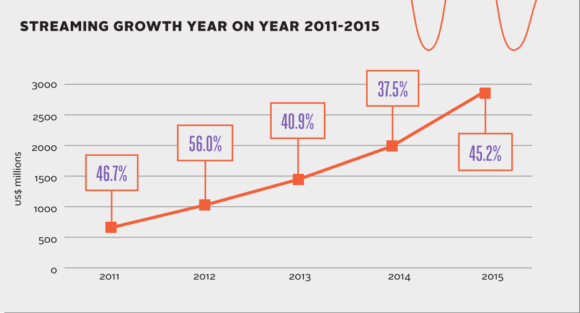
\includegraphics[width=0.7\textwidth, natwidth=580bp, natheight=313bp]{figures/ifpi_stream_growth.png}
    \caption{IFPI's streaming growth report}
    \label{fig:ifpi-growth-report}
\end{figure}

	Music streaming follows this trend of growth on the latest economical reports. Over the five year period to 2015, the observed revenue from the industry grew four times to US \$2.89 billion as can be seen in Figure \ref{fig:ifpi-growth-report} from the IFPI organisation \citep{ifpi}. The increase in the number of paying subscribers is also of notice, seeing an increase from 8 to 68 million people over the same period. This new model also helped bring some countries where licensed music market was losing ground to piracy like China and Mexico, and it corresponds to around 20\% of the industry's revenue in the top five markets in the world. 
	
	\subsection{Spotify and the growing competition}	
	
	\begin{figure}[h]
    \centering
    
\includegraphics[width=0.3\textwidth, natwidth=506bp, natheight=900bp]{figures/spotify_screenshot.png}
    \caption{A screenshot of Spotify's Android app}
    \label{fig:spotify-screenshot}
\end{figure}
		
	Spotify is the top music streaming service globally in terms of number of users, totalling 100 million of which 50 million are Premium paid subscriptions \citep{spotifypress}. The content is delivered through applications available on several different operating systems like Windows, macOS and Linux, as well as devices like iOS and Android tablets and smartphones, an example is shown in Figure \ref{fig:spotify-screenshot}. Users may access over 30 million songs available in its catalog through two methods: a free membership where the client is exposed to advertisement, and a Premium paid subscription with additional features like offline downloads, increased music quality and unlimited number of song skips. Spotify also is well known for its music recommendation subsystems like Discover Weekly and Daily Mix that provides playlists tailored to each user based on their listening history. The service is available in most of Europe, as well as in Australia, New Zealand, most of the Americas and several Asian countries.	
	
	The promise of growth in the area however has attracted well known brands to the dispute like Apple and Google, and their growth, while still not up to par with the top players, has been steady and may be significant in the following years \citep{ifpi}. The market is becoming saturated with competition, and any contender to the top position in the music streaming area must strive to keep its current user base at all costs. The loss of a customer, be it for the competition or not, is called in the industry as \emph{churn} and is commonly seen as a metric that should be minimized in a customer relations framework (CRM) of a service provider. For that goal, an important step is to identify prematurely the candidate churning customers and to leverage actions that may avoid them from leaving, and this is commonly achieved by making use of the wealth of historical information that digital providers have about their users. 
	
\subsection{Churn prediction}	
	
	\emph{Churn prediction}, the task of identifying the most probable churning customers of a service provider, is an established topic in the literature and has seen a considerable amount of research specially on the mobile telecom industry \citep{Hassouna2015} \citep{Lu2014} \citep{Khan2015}.  Several classical techniques for predicting churn like decision trees and logistic regression have been used on recent work \citep{mahajan2015review}, however most of them make use of user behaviour data at a single point in time, normally the most recent one when the dataset was created. The user is commonly represented by summarizing or aggregating his behavioural feature values over a fixed time window, thus losing any latent sequential information that might be contained in the data set. This is a simplification that eases the burden of training a predictor model since the customer data is commonly high-dimensional and difficult to work with, nonetheless latent attributes, when used properly, have been shown to improve significantly a predictor's performance for industries like mobile telecom \citep{GurAli2014}.
    
    Intuitively one can think that latent factors hidden in the temporal axis of the user behaviour data could yield a better prediction accuracy when comparing to a model which leverage a single and static point in time. For instance, a user that is gradually reducing its consumption of the service over time can be easily thought of a prospect churner. While this intuition is trivial to come up with, we are also interested in learning strong correlations between temporal aspects of the data and the churn rate which are not as clear to the eye. Our hypothesis is that making use of the properties hidden on user behaviour data over time, a churn rate predictor could improve its accuracy greatly when compared to methods which are static on time.
    
\subsection{User retention}    
    
A churn rate predictor which can identify possible churners accurately is just a trigger on the user retention process that can span several different stages. One of these stages is to identify what actions can be taken by the service provider as to avoid the user abandoning the service. An important problem to solve beforehand is to identify which features of the data have a strong statistical correlation with the churn rate. With that information, the providers could for example set up automated actions as to influence the value on these features. Learning which are the most important features is also of relevance for the task of choosing what data to use for training the predictor models, since commonly service providers have a vast amount of data about the user but only a fraction of that is of importance for predicting churn: training models with a full dataset will commonly introduce error on the system and take a large amount of computing resources to train.
	
\subsection{Objective}	
	
The goal of this project will be to research different models for churn prediction that can make use of the temporal aspect of user behaviour data at its fullest. Our hypothesis is that latent factors hidden on usage patterns may increase the accuracy of state-of-art predictors which considers only the state of the data at a single point in time. We shall experiment on different models that are known to perform well on time series data and compare their accuracy using different evaluation methods. Detecting possible churners, while important, does not improve user retention without an associated action performed by the service provider. To derive insights on what can done to improve this metric, a deep data exploration and feature analysis is also a goal of this project. Features shall be correlated to their influence on the churn rate, and feature selection techniques shall be researched and implemented in an attempt to reduce bias on the churn classifiers.    

\chapter{Background}

TODO: write intro paragraph

\subsection{Definitions}

\newtheorem{definition}{Definition}

\begin{definition}
A \emph{session} is defined as the time period the user is engaged into the application, be it to stream music or to navigate through the available content. A session starts when a user interaction trigger is captured (eg. a button click), and the session ends when no such trigger is captured and no continuous activity is being performed (eg. listening to a song) for at least 15 minutes.
\end{definition}

The session is the basic measurement of activity of the user on the service. Users are considered \emph{active} if they are currently on a session, and \emph{inactive} otherwise. (TODO Check Sahar)

\begin{definition}
A user is defined to have \emph{churned} if no session of his was registered in the last 30 days.
\end{definition}

Note that this definition is not concerned whether the user is a paying customer or not, but only if he is actually making use of the service. For example, a user may be subscribed to a Premium paid account and still be considered to have churned if no activity was registered in the last 30 days. However, it should be noted that empirical observations by the service provider suggest that there is a significant behavioural difference between the two classes of users that will be taken into consideration when the experiments are performed. (TODO Check Sahar)

\subsection{Feature Selection}

TODO: add feature selection techniques (Information gain, L1-norm, Recursive Feature Elimination, Variance Threshold...)

\subsection{Predictor Models}

\subsubsection{Logistic Regression}

Logistic regression is a linear regression model used to predict the probability of occurrence of a categorical variable, like the churning and non-churning labels. First developed by mathematician David Cox \citep{cox1958regression}, this technique has been used in wide range of domains like medical fields, marketing and economics (TODO: add refs?), and is as of today one of the most used models for predicting the churn rate of customers on the telecom industry \citep{mahajan2015review}. Despite its name, logistic regression is used mostly as a classification algorithm, since its output is a probability score that together with a threshold can map the input to one of the supplied labels (churn and no-churn, for example).

The premise of logistic regression is that the output variable $y$ can be modelled as a linear probability function dependant on a set of input feature values  $\bm{x} = [x_1, x_2, ..., x_n]$ through a set of equations that follows:

\begin{equation}
p(y = 1|\bm{x}) = f(t)
\end{equation}

\begin{equation}
f(t) = \frac{1}{(1+e^{-t})}
\end{equation}

\begin{equation}
t = w_0 + w_1x_1 + ... + w_nx_n = \bm{w}^T\bm{x}
\end{equation}

where $y$ is the true output variable that can take the values 0 or 1 in a binary classification problem. $t$ is a linear combination of the input $\bm{x}$ with a trainable weight vector $\bm{w}$. $f(t)$ is the logistic function that gives name to the model. This function has the property of "squashing" any real input to a value between 0 and 1, and thus it can be interpreted as a probability. 

TODO: add models (Decision Trees, Logistic Regression, Random Forests, LSTMs, CNNs...)

\subsection{Evaluation Metrics}

\subsubsection{Confusion Matrix}

A \emph{confusion matrix} (also called contingency table) is a table layout representing the performance of a classifier's output, judging by its predictions against the actual true values. In a binary classification problem, the confusion matrix is a 2 x 2 table where commonly the rows represent the true labels while the columns the predicted classes. Each cell contains a count of how many samples were classified on that category, and the values in the diagonal represent the correctly classified samples (if the features are ordered). Table (TODO: Add table) depicts a confusion matrix for a binary classifier.

The confusion matrix is an excellent visualization tool to estimate the performance of a model. The values that should be maximized, the \emph{true positives} (TP) and \emph{true negatives} (TN), represent the samples that were correctly labelled as possessing the feature of interest or not, respectively. On the other hand, the \emph{false positives} (FP) and \emph{false negatives} (FN) are the misclassified samples where the algorithm predicted that the feature was present while in truth it was not and vice-versa. In this work, the positive class will always represent a churning user, and it follows that the negative class represents the non-churners.

\subsubsection{Classification Accuracy}

Several different metrics can be derived from the confusion matrix table. The \emph{classification accuracy} (CA) of a model is a common metric that corresponds to the fraction of the correctly classified samples on the test set, and can be calculated as follows:

\begin{equation}
CA = \frac{TP + TN}{TP + TN + FP + FN} 
\end{equation}

While trivial to understand, this metric may lead to erroneous conclusions when class imbalance is present in the test set, which is a common occurrence on the churn prediction domain. For example, if 9 out of 10 users of a dataset are non-churners, any classifier that simply outputs a negative class for all samples will result in an accuracy of 90\%, however its ability of detecting churners is non-existent. For a service provider, detecting churn cases is always more important than detecting the loyal users, and this metric by itself cannot represent this goal. (TODO Add ref? Hassouna 2015)

\subsubsection{Precision, Recall, Fall-out and False Alarm}

To address the class imbalance problem of the classification accuracy, others metrics are also commonly used. The \emph{positive predictive value} (PPV, also known as precision) is the proportion of the samples labelled as positive which are true positives, and describes the performance of the algorithm. The \emph{true positive rate} (TPR, also called sensitivity and recall) of a model corresponds to the number of correctly predicted positive samples divided by all positive samples. \emph{True negative rate} (TNR, also called specificity and fall-out) is the number of correctly predicted negatives divided by all true negatives. The \emph{false positive rate} (FPR, also called false alarm ratio) is the probability of receiving a false positive as output of an experiment, and is calculated by dividing the number of false positives by the total number of positive samples.

\begin{equation}
PPV = \frac{TP}{TP + FP}
\end{equation}

\begin{equation}
TPR = \frac{TP}{TP + FN}
\end{equation}

\begin{equation}
TNR = \frac{TN}{TN + FP}
\end{equation}

\begin{equation}
FPR = \frac{FP}{TN + FP} = 1 - TNR
\end{equation}

Depending on the distribution of classes of the dataset, it is often difficult (although desirable) to maximize both metrics at the same time. A compromise must be reached that achieves the best trade-off between the two, which is commonly a business decision. For a music streaming service like Spotify, maximizing sensitivity is preferred due to the costs associated with a churning user, however a reasonable specificity is also a metric that should be strived for. (TODO Check with Sahar)

\subsubsection{Receiver Operating Characteristic}

The \emph{receiver operating characteristic} (ROC) is a visualization tool that plots the relationship between the true positive rate (commonly the y-axis) and the false positive rate (the x-axis) of a binary classifier system. The curve is drawn by selecting different parameters of a model or levels of threshold for the decision boundary between the positive and negative classes. For example, when the output of a classifier is a probability value (like in logistic regression), different thresholds can be chosen to decide whether a user is a churner or not, depending if the goal is to minimize FPR or maximize TPR. An example of a ROC curve can be seen in Figure (TODO Add figure)

A good classifier would score values close to the upper-left corner of the plot, where the point (0,1) represents a perfect classifier with 100\% TPR and 0\% FPR. On the other hand, an algorithm that outputs a curve alongside the diagonal where TPR and FPR are almost the same at different threshold levels can be considered close to a random guess, like the flip of a coin. A classifier would underperform if its scores are closer to the bottom-right corner of the plot, however this result can always be mirrored by updating the model to simply invert the positive and negative labels of the classified samples.

ROC curves can be used to compare the performance of different models by measuring the \emph{area under the curve} (AUC) of its plotted scores, which ranges from 0.0 to 1.0. The greater this area, the better the algorithm is to find a specific feature. Moreover, models with an area close to 0.5 can be assumed to perform not much better than random guess, since this is the total area under the diagonal line.

TODO: Add eval methods (F-score, Lift chart, Top Decile Lift (TDL)...)
\chapter{Related Work}

TODO: write intro paragraph

\section{Churn Prediction}

Identifying which users are most likely to churn is an important step in any customer relationship management (CRM) framework interested in improving user retention. It has been shown that several economical values are directly correlated with the customer lifetime metric that can be crucial in a competitive market, like how the costs of acquiring new customers surpass those of retaining existing ones and how loyal users usually spend more and can bring in new customers \citep{GurAli2014}. Thus, churn rate prediction is an established topic in the literature and has seen studies being performed on a wide range of domains like the telecommunication industry \citep{Lu2014}\citep{Khan2015}\citep{Hassouna2015}, social multiplayer games \citep{Borbora2011}\citep{Runge2014} and community-based question answering services (CQA) \citep{Pudipeddi2014}\citep{Dror2012}. 

The very first aspect of the study that any researcher has to take into consideration is the formal definition of what churn is, which depends on the domain that the data set belongs to. \citep{lazarov2007churn} divides the definition into three types: \emph{active} where the contract is officially terminated, \emph{hidden} when the customer is inactive (not using the service) for a significant amount of time, or \emph{partial} when the customer is not using the service at its fullest, opting for a competitor instead. Subscription-based services like mobile companies \citep{Lu2014}\citep{Hassouna2015} and massive multiplayer games \citep{Borbora2011} commonly utilizes the active churning definition caused by the explicit termination of the agreement. Social games \citep{Runge2014}\citep{Drachen2016RapidPO} and CQA services \citep{Pudipeddi2014}\citep{Dror2012} however usually model the user interest by measuring its level of activity and engagement since no contract is formally established, opting for the hidden churn definition instead. 

Even though Spotify has a contract-based Premium service, this project is interested in the clients who are inactive for some time, whether they are paying customers or not. Delving into the hidden churn definition, one could ask what is considered a "significant amount of time" as to judge a user to have churned or not, and different domains have distinct approaches depending on the way the interaction between user and service takes place. For example, for a mobile network like the one studied in \citep{Khan2015} this definition can span months of inactivity since customers on that market are commonly more loyal, even though this paper focus on pre-paid accounts with "soft" contracts. On the other hand, rapid-changing markets like free-to-use services as social games and CQA sites prefer to define the churn period as small as possible (commonly days or weeks), since the absence of an agreement makes it easy for customers to switch for the competition, having the service the obligation to act faster if any sign of loss of users is identified \citep{Khan2015}\citep{Drachen2016RapidPO}. On \citep{Dror2012} the focus is set on new users so the the churn period is explicitly set to be their first week of activity. \citep{Pudipeddi2014} however focus on both new and experienced users by considering the first days and posts (questions and answers) as parameters on the models trained, evaluating each independently.

Current literature for prediction of churn rate uses a wide range of machine learning technologies, such as decision trees \citep{Pudipeddi2014}\citep{Hassouna2015} \citep{Ballings2012} \citep{Khan2015}, logistic regression \citep{GurAli2014}, neural networks \citep{Runge2014} and its convolutional variant \citep{Wangperawong2016}, random forests \citep{Dror2012} and support-vector machines \citep{coussement2008churn}. The number of techniques is vast, however it can be mentioned that current research suffers from a difficulty to reach insights that can generalize well for other areas, since the applications that the data sets belong to are domain-specific, greatly influencing how the users interact with the service. Interpretability is a key component in any application since the end goal is always not only to detect the users most likely to defect but also the reasoning behind their departure, as to plan reasonable actions to increase retention. With that in mind, even though some models like weighted random forests \citep{Burez2009} and neural networks \citep{Runge2014} offer a higher accuracy for some domains, the difficulty in getting key drivers behind the consumer's behaviour in some "black-box" type of models have led to researchers opting for a more interpretable technique like logistic regression which is commonly a close second place in terms of performance \citep{Runge2014} \citep{Dror2012}. For that reason, decision trees and logistic regression are as of today the most popular techniques for churn prediction, yet a consensus of the best model cannot be reached by researchers as stated by \citep{mahajan2015review}. 

The telecom industry is by far the most well researched area for predicting churn, and a proper review would be incomplete without mentioning some examples. In \citep{Hassouna2015}, two popular models for predicting user churn were empirically compared: decision trees and logistic regression. By making use of the data set provided by a mobile operator, two models were created by independently training and selecting their best performing versions. Evaluation was executed by comparing the AUC of their ROC curves, as also their Lift score and overall accuracy. The conclusion is that decision trees consistently perform better when compared to logistic regression models, and thus should be a preferred choice. In \citep{Lu2014}, churn classification was performed on users in a rather unique way. The Gentle AdaBoost boosting algorithm was used alongside a logistic regression base learner as to train a model to do the separation between the churning and non-churning classes. However, one further step was performed where the users were split into two clusters based on the weights assigned by the boosting algorithm. One of the clusters was identified to have a considerably larger churn rate than the other, and thus another logistic model was trained using the clusters as labels, and its performance evaluated using ROC curves. The idea behind this approach is to use a model to mark users who have a high risk of leaving the service (and be the focus of user retention actions), instead of labelling them as churners and non-churners directly. On \citep{Khan2015}, billions of call detail records from a mobile phone operator was the focus of a churn prediction study and feature analysis. The initial data set was filtered to the calls made by 100.000 subscribers during a 6 month period. A brute-force approach to feature engineering was then performed to create 12.914 out of the initial 10 features by combining every feature from each of the manually split 8 different groups. Feature selection is then performed in two distinct ways: first, an individual Student's t-test score is computed for each individual feature to evaluate how well it can differentiate between the churners and non-churners sets. Second, a tree-based method was used as to estimate the the accuracy of a joint classifier by adding features one at a time. Features are then ordered by their statistical correlation with churn, and the top 100 features were selected to train several different classifiers. Evaluation was performed mainly by comparing the AUC of each model, where AdaBoost using a decision tree classifier performed the best, followed closely by a logistic regression model.

The rapid increase in Internet popularity has spawned a plethora of new services in the last decade, and thus a wider range of domains like CQA sites and gaming applications are being researched for churn prediction. In \citep{Dror2012}, an explorative study was made on the Yahoo! answers website as to discover an efficient churn predictor model and also the features that correlates with the user leaving the service, however differently from other works this paper focused on new users with less than a week of activity on the service. Features were grouped into Question, Answer and Gratification categories, and were used for training several different classifiers. For this dataset, random forests performed the best with logistic regression as close second. Features were also ordered by the amount of information gain that they provide, and the number of questions and answers are the top features on that regard (inversely correlating with churn), followed by the period of time the user is active and gratification features for answers given and questions made. In \citep{Pudipeddi2014}, the younger CQA service Stack Overflow was the focus of a study on user behaviour characterization and churn rate prediction. An extensive data exploration was made as to correlate features to the chance of a user leaving a service, and with those insights classical modelling techniques were used, where the best performing one was a decision tree. The approach used for extracting and categorizing features (temporal, frequency, gratitude, etc) and the insights that follow the study (like the importance of temporal features for predicting churn) is of high value and can be mapped to concepts on a different domain like a music streaming service with minor modifications. 
In \citep{Runge2014}, players responsible for generating the most profit on two casual social games were the focus of a study on churn analysis and prediction. Formal definitions for active players and churning were made, and the problem was defined as a binary classification task where users were labelled as leaving the service or not in the following week of when the models were trained. Four different models were then trained, and a neural network classifier obtained the best area under the curve (AUC) score, with logistic regression as a close second. The formal definitions of "churn" and "activity" can be applied to a music streaming service in a similar way, as the evaluation of performance using a series of receiver operating characteristic (ROC) curves. In \citep{Borbora2011}, the activity log of a subscription-based multiplayer online game was the source of an experiment focused on comparing two different methods for predicting the users with a higher tendency to leave the service, a theory-driven and data-driven approaches. For the modelling, an ensemble method was used with several different classifiers, where the choice of model was made based on whether the cluster of the data set (found with K-means) that will be used to train the classifier has a significant proportion of churners or not. Even though the performance of the data-driven model was superior, the difference was negligible when taking into consideration the complexity of the models and also its interpretability. Moreover, if marketing resources are constrained the theory-driven model was considerably superior for the first 40\% of users on the lift chart. 


\section{Sequential Modelling for User Behaviour Data}

Even though there is currently a wealth of research on churn prediction techniques, most of them treat the user behavioural features as static points in time by aggregating or summarizing their values over a time window \citep{Auon2015}. It is a simplification that eases the hassle of training models with a data set which is commonly high-dimensional and difficult to work with, however information that could be used to improve the predictors' performance is lost in this process  \citep{GurAli2014}. For example, there is no information as to when over the time window being analysed a user decides to churn, it could be that all defectors are grouped into a period where an external event (like the end of an offer) has taken place. Environmental variables, that is those that varies through time but are common to all users, are also omitted on static models, leaving it to the experts the task of manually integrating these features on their analyses. Newer models like \citep{Pudipeddi2014} attempt to integrate some temporal data by manually engineering features related to time (like the duration of an event, for example), however since each user is represented as a sample in a single point in time the sequence of data transformations is inherently lost in this process.

It is natural to think that the human behaviour evolves through time. Our opinions and desires changes in accordance to the stimuli that we receive from the world around us, and summarizing our persona by looking at a single point in our life is an oversimplification that does not make justice to the path that leaded us to where we are. Dealing with temporal data is by no means trivial however, and to leverage fully its properties some careful considerations about this type of data must be done. On \citep{Langkvist2014}, an overview of the challenges on creating models that make use of the time component on data sets are presented to the reader. Also, since hand-crafted features are generally domain-specific and difficult to create, a review of the current research on unsupervised feature learning applied for time-series data is the focus of this paper. From the challenges, it is worth of mention the uncertainty that there is enough information to understand the underlying process, its non-stationary characteristics like mean, variance and frequency, and its common high dimensionality and noise. The right representation is deemed then crucial for any model to be successful in its goal. Several different techniques currently being used for unsupervised feature learning are then presented in details to the reader, where it is worth of quick mention the conditional Restricted Boltzmann Machine (cRBM), Recurrent Neural Networks (RNN, with is Long Short-Term Memory extension), the Gated RBM, the Time-Delay Neural Networks, and the Space-Time Deep Belief Network. Finally, several classical time-series problems are reviewed alongside the best models currently being used for each domain. 

The hypothesis that sequential patterns hidden on temporal data can improve the accuracy of predictor models is not an uncharted territory however, and has being recently explored by researchers on similar domains as churn prediction that could be mapped to with minor modifications. Sparked by positive results of recurrent neural networks on domains like speech recognition \citep{graves2013speech} and video classification \citep{yue2015beyond}, some papers attempt to recreate similar deep architectures on their own prediction problems. On \citep{Tax2016}, a technique was presented as to predict the next event and its timestamp on a running case of a business process (a help desk process, for example). Three different LSTM architectures were experimented on, one for each of the problems being tackled: estimating the next activity and its timestamp, all the remaining activities in a use case and the remaining time of a process. This technique could be used for churn prediction by interpreting the user interaction with the service as actions, and "churn" could be an event that may or may not exist in the process chain. The LSTM architecture was also present on \citep{Auon2015} alongside a quantile regression (QR) model as to predict which of the past buyers of a store chain will return after acquiring a product on sale. The hypothesis is that a performance gain can be achieved by combining models that are know to perform well on both temporal and aggregate features, respectively. It was empirically shown that a mixture of experts approach between these two techniques can reach a significant mean-square error improvement when comparing to any of the models when evaluated independently. 

Deep architectures like LSTMs could theoretically be applied in a similar way for the task of predicting which users are more likely to abandon a service, however the lack of research using techniques like these suggests that this mapping may not be as easy as it seems, nevertheless some examples can still be found in the literature. Inspired by results obtained on image recognition \citep{krizhevsky2012imagenet}, a convolutional neural network (CNN) model was used as a churn predictor on the work by \citep{Wangperawong2016}. On it, users were represented as 2-dimensional images where columns are the tracked features and rows are days organized in sequences. Two different CNN models were used, and both outperformed a baseline decision tree model. On \citep{GurAli2014} the researchers propose a new data set generation framework that can better leverage the temporal aspect of user behaviour data for churn prediction models. The hypothesis being tested is that by boosting the data with features on different time periods instead of only the last one, a significant performance gain can be achieved. The main framework of this study is called Multiple Period Training Data (MPTD), which basically consists of aggregating to each user their features at each predefined time step along the time range of the data set, alongside their churn labels at each point in time and also environment variables which varies through time but are common for all users. This framework was tested against a classical static data set, demonstrating a significant improvement (by \emph{p-value} comparison) on AUC and TDL for both logistic regression and decision tree models for predicting if the user is going to churn on the next test period or nor. Another experiment was focused on predicting churn several periods on the future, and for that a common survival analysis method called Cox regression was used as a benchmark for comparison against logistic regression models trained on MPTD. It was empirically concluded that using several independently trained binary classifiers, each trained on a different parameter to the "churn within $\delta$ periods" (W$\delta$C) feature, a significant performance gain can be achieved when comparing their respective AUC and TDL.


\section{Evaluating and Training Churn Prediction Models}


Data sets from service industries often have a common characteristic that may be problematic while training models, which is the uneven distribution between the churning and non-churning classes. It is a common scenario for the number of non-churners to heavily outweigh the number of churning samples on real data sets. Class imbalance is thus a recurrent concern in almost all domains, however research in this area lacks the proper attention. \citep{Burez2009} aims to solve this mystery by focusing entirely on how the uneven class distribution affects the performance of several different classifiers. The performance boost estimated to be received by using a cost-sensitive learning algorithm (where false negatives are assigned a greater cost than false positives) is also evaluated, and it has taken the form of a weighted random forest model which was compared to other classical baseline models like logistic regression and random forests. Under-sampling, where fewer samples from the majority class are incorporated in the training data as to artificially change the distribution between the labels, is proved to significantly improve the performance of the underlying models, however the exact ratio between churners and non-churners is confirmed to be case-dependant, not necessarily being the even distribution the perfect choice. 

To deal with the problems brought by the unbalanced distributions mentioned above, proper evaluation metrics must be used as to avoid the predictors to be biased towards the majority class. It is a well know fact that the accuracy of a classifier is not an appropriate method when comparing the performance of different models \citep{powers2011evaluation}, and so no paper reviewed used this metric by itself. The overwhelming majority of the literature abides by the use of AUC as a proper metric for predicting churn rate, \citep{Ballings2012} \citep{GurAli2014} \citep{Khan2015} \citep{Lu2014} to name a few. \citep{Burez2009} delves into this topic and defends the use of AUC as a proper metric, while adding the cumulative gains chart as to graphically represent the percentage of customers has to be targeted to reach a percentage of churners. The F-score is also sometimes added as a metric of interest, normally in conjunction with AUC \citep{Dror2012} \citep{Khan2015}. In respect to graphical representations, ROC curves and lift charts dominates the literature as appropriate methods, and it is present in works like \citep{Lu2014} and \citep{Burez2009}. 

Another question that can be made is how far in the user history models must be trained on as to achieve the best trade-off between accuracy and computational burden. It is intuitive to imagine that user actions far in the past exerts little influence on predicting whether the user is going to churn or not in the near future, however the exact threshold that should be used is not trivial to find. \citep{Ballings2012} attempts  to answer this question by experimenting with three different models (logistic regression, decision trees with and without bagging) on a newspaper data set consisting of 16 years of user history. The models were evaluated for their performance by training with data ranging on this interval with a 1-year gap between each measurement. It has been concluded that  after year 5 no gain in performance (measured by AUC) is statistically relevant enough to warrant the increase in computational power needed for the training. However, the researchers also question whether this result can be extended for other domains or not, leaving that for future work.

Current data sets from service providers have no lack of user historical information stored, however the probability that all available features have a significant correlation to churn rate is pretty slim. Using too many features may lead to undesirable effects like overfitting and falling into the "curse of dimensionality" problem, reducing the classifiers performance as cited by \citep{guyon2003introduction}. It is a common step to pre process the data in a way as to mitigate this risk, but still there is no single method in the literature that dominates the scene. Several papers do a manual subset selection of features based on theories, testing each using baseline classifiers and selecting the subset with the best performance \citep{Pudipeddi2014}\citep{Runge2014}. Others works like \citep{Borbora2011} and \citep{Dror2012} use information gain as a metric to classify the features on their expected reduction in entropy. One step further is taken by works like \citep{Lu2014} and \citep{Khan2015} where full decision trees are built specifically for feature selection. Another more exotic method was used by \citep{Wangperawong2016} with an autoencoder to discover which features influenced the churn rate the most. 

Churn prediction has been explored in different kind of applications on recent literature, however music streaming services are as of today a quite under-researched area, even though there is a prominent feature that makes it significantly different from other more researched and similar areas like video streaming, which would be the absence of the constant attention factor that video demands. Studying the user behaviour in each application can possibly help optimizing parameters that are difficult to tune without expert knowledge on how the interaction between costumer and application occurs. The work by \citep{Zhang2013} aims to fill that gap by analysing patterns of usage of Spotify's Premium subscribers on features like session and playback arrival patterns, user behaviour on single and multiple devices and favourite times of day for streaming. The main contributions of the study can be summarized as follows: First, daily patterns can be observed on features like session arrival, playback arrivals and session length. Second, there is a high probability of users to continue on the same device for consecutive sessions. Third, users have their unique times of day when they prefer to stream music on the platform. Fourth, a session length can be used as a good indicator of the next session length and also downtime.


\chapter{Methods}

* Baseline classifiers (Decision Trees, Logistic Regression, Random Forests?)

* Temporal classifiers (LSTM, CNN?)

* One classifier vs different values of class distribution (skew)

* Different subset of features


\chapter{Results}

\lipsum

\chapter{Conclusions and Future Work}

\lipsum[5]

\bibliography{references}

\appendix

\chapter{Unnecessary Appended Material}

\end{document}
